\documentclass[manuscript=cmatex]{achemso}
\usepackage[usenames,dvipsnames]{xcolor}
% \definecolor{linkcolor}{RGB}{0,0,240}
\usepackage{achemso}
\usepackage{makecell}
\usepackage{xr-hyper}
\usepackage{hyperref}
\usepackage{hypcap}
\usepackage{appendix}
\usepackage{upgreek}
\usepackage{chemmacros}
\usepackage{siunitx}
\usepackage{textcomp}
\usepackage{natmove}

\captionsetup{font={rm,small}}
\SectionNumbersOn
\usechemmodule{reactions}
\chemsetup{modules=reactions}

\usepackage[USenglish]{babel}
\addto\captionsenglish{\renewcommand\chaptername{Section}}
\usepackage{graphicx,array,tabularx,mathtools,siunitx,amsmath,multirow,longtable,float}
\usepackage[nameinlink,noabbrev,capitalize]{cleveref}
\setlength{\footskip}{0.25in}
\usepackage[labelformat=simple]{subfig}
\graphicspath{ {./imgs/} }
%\usepackage[version=4]{mhchem}
\usepackage{cleveref}
\usepackage[labelfont=bf]{caption}
\hypersetup{
  pdfstartview = {XYZ},
  allcolors = linkcolor,
  bookmarksopen,
  bookmarksnumbered,
  colorlinks=false,
  filecolor=black,
  citecolor = black,      
  urlcolor=black,
}

%%%%%%%%%%%%%%%%%%%%%%%%%%%%%%%%%%%%%%%% 
%%%%%%%%%%% 
% \numberwithin{reaction}{section}

\makeatletter
\@ifundefined{ignorespacesafterend}{\def\ignorespacesafterend{\global\@ignoretrue}}{}
\newenvironment{subreactions}{%
  \refstepcounter{reaction}%
  \protected@edef\theparentequation{\thereaction}%
  \setcounter{parentequation}{\value{reaction}}%
  \setcounter{reaction}{0}%
  \def\thereaction{\theparentequation\alph{reaction}}%
  \ignorespaces
}{%
  \setcounter{reaction}{\value{parentequation}}%
  \ignorespacesafterend
}

\externaldocument[supp-]{si}

\makeatother
\title          {Evolution of Copper Surfaces under Plasma Oxidation: Molecular Dynamics Study with Neural Network Potentials}
\author         {Yantao Xia}
\affiliation    {Department of Chemical and Biomolecular Engineering, University of California, Los Angeles, CA 90095, USA}
\email          {xyttyxy@ucla.edu}
\author         {Philippe Sautet}
\affiliation    {Department of Chemical and Biomolecular Engineering, University of California, Los Angeles, CA 90095, USA}
\alsoaffiliation    {Department of Chemistry and Biochemistry, University of California, Los Angeles, CA 90095, USA}
\email          {sautet@ucla.edu}

%%%%%%%%%%%%%%%%%%%%%%%%%%%%%%%%%%%%%%%%%%%%%%%%%%% 
% table formatting commands
\renewcommand{\thesubfigure}{\relax} % no labels on subfigures
\begin{document}
\abstract
The formation of thin oxide films is of significant scientific and practical interest. Among the various metals, Cu is one of the most intensively studied. However, in contrast to heavy efforts, little progress had been made in understanding the fundamental mechanisms of this seemingly simple phenomena. The major limiting factors inhibiting theoretical progress are identified to be the length and time scale issues. In this paper, a neural network potential is trained using data generated using density functional theory (DFT) and applied to study the impact of oxygen atoms and molecules on Cu (100) surfaces. The dynamic of diffusion and film growth is accelerated using collective variable hyperdynamics (CVHD). Using these tools, we explored the initial and late stages of oxide growth. The effect of temperature and, in the case of plasma oxidation, ion kinetic energy, is explored in detail \textbf{[Replace with actual results when you have them]}.

\section{Introduction}
\label{sec:intro}

After replacing aluminum decades ago, copper became the universal material of choice for interconnects in integrated circuits. Traditionally, copper was introduced into the back-end-of-line (BEOL) processing by a combination of the Damascene wet plating and the chemical mechanical polishing (CMP) processes. However, continued down scaling in the relentless push to follow Moore's law is beginning to render this harsh process unsuitable at the lowest levels of metallic interconnects. 

In response to these problems, the semiconductor industry is actively looking for an atomic-level engineering approach capable of achieving high-selectivity simultaneously. One of the most promising techniques is atomic layer etching (ALE). To etch metallic copper, a specific variant, the plasma-thermal ALE process is used. It is composed of two self-limiting steps (Figure \ref{fig:scheme}): 1) conversion of surface layers of copper to copper oxide under oxygen plasma and 2) reaction of the oxide layer with the etchant molecules (\textit{e.g.} \ch{HCOOH}) to form volatile complexes. While plasma is required to impart the inherent directionality from the electric field-accelerated ions to devices, the accelerated ions lead to relatively thick, non-self-limiting activated layers (compared with thermal ALE), preventing the process from achieving a finer grain of control over etch per cycle (EPC). 

Copper oxide is one of the enabler materials of modern technology. Stable at ambient conditions with an optimal band gap of $\sim \SI{2.0}{eV}$, it is a highly desirable and readily available material for photocatalysis and photovoltaic cells. Incidentally, the oxidation of copper is one of the most heavily studied oxidation processes of copper. The Cabrera-Mott theory of metal oxidation was conceived of partially as an explanation for the formation of thin copper oxide films. While the classical theory was shown to be inaccurate as understanding improved, it brought an immense interest to the phenomena to the point where copper oxidation is considered a model system to understand formation of thin metal oxides, in the hope that the fundamental understanding can be transferred to other metal surfaces.\cite{gattinoni_atomistic_2015}

The oxidation of low-index copper surfaces has been extensively studied under surface science conditions. Oxygen is known to adsorb dissociatively on the (100), (111), and (110) terminations, forming well-characterized configurations and reconstructions at temperatures below the room temperature. As coverage increases, the oxide grows as nanoislands on all three terminations, as opposed to the uniform layer growth assumed in earlier works. The size and shape of the islands depends on the surface, the conditions, and the oxygen dose. In the conditions removed from the ultra high vacuum to the more realistic pressures, temperatures, and time scales, the process is far less well understood. There is little concensus on the form of the rate law at temperatures near or above room temperature, and we still do not understand well the thickness and the composition of the native oxide, nor the influence of temperature, moisture, \textit{etc}.

In addition to the difficulties that makes understanding thermal oxidation challenging, the interaction of metal surfaces with the plasma is unique in having energetic particles impacting the surface. The particles used in processing has energies on the order of \SI{10}{eV}, high above those possible from thermal fluactuations, yet too low to cause ion implantation. As the energy is within an order of magnitude of the strength of a typical chemical bond, the subtleties interplay of chemistry are still preserved, however at much higher rates than those attainable thermally. 

To the author's awareness, there have been no molecular dynamics studies on the interaction between a metal surface and the low-temperature plasma. Existing surface-plasma interactions almost always involve \ch{Si}-based materials, and are performed with classical interatomic potentials (\textit{e.g.} Tersorff-Brenner \& Stellinger-Weber). These simulations set the ground for computational studies of surface-plasma interaction at the atomic scale, but they are fundamentally limited in accuracy by their functional forms, and cannot be used to capture the subtle chemistry at the intermediate energy ranges. Recent development of bond-order based reactive force fields (\textit{e.g.} ReaxFF and Charge-optimized manybody potential (COMB)) have been applied successfully to the thermal oxidation of copper, but their functional forms prevent the accurate description of the regions of the potential energy surfaces encountered during plasma oxidation. The recent development of machine learning potentials such as the Behler-Parinello high dimensional neural network potentials (HDNNP) and the gaussian approximation potentials (GAP) provide functional forms that are versatile enough to be parametrized to describe highly diverse chemical environments at or near the accuracy, previously only achievable with expensive first-principles calculations. 

\begin{figure}[h]
  \centering
  \includegraphics[width=0.7\textwidth]{scheme}
  \caption[Overall process of plasma-thermal ALE on \ch{Cu} metal]{Overall process of plasma-thermal ALE on \ch{Cu} metal}
  \label{fig:scheme}
\end{figure}

% some information on the thermal oxidation. but the focus of this paper is plasma oxidation
% 
% experimental:
% TGA, macroscopic
% EM/TEM/variants: nanoscale imaging but not surface specific
% these are electron imaging techniques, measuring the number and intensity of transmitted/emitted electrons
% STM: surface specific. This is not an electron emission/transmission based technique. Rather it measures the tunneling current, still electrons but a different mechanism
% atomic composition and oxidation states can be obtained using XRD, AES, EELS, LEED. These are diffraction techniques that have high spatial resolution, but applies only to periodic systems hence typically work only on thick films / bulk material

% the reaction sequence leading to oxidation of a clean metal surface is generally accepted to be oxygen chemisorption, nucleation and growth of the surface oxide, and bulk oxide growth

% O2 adsorbs dissociatively at room temperature on Cu(100),(110) and (111), with barriers of 0.1 eV for (100), 0.1 - 0.3 eV for (110) and 0.1-0.2 eV for (111).
% These barriers are DFT values, using some archaric method I'm asking Ziyang about
% At below 50K and 100K, O2 binds molecularly on (100) and (110), respectively.
% This is what I've observed with my NNP as well

% XAFS on Cu(100): molecular adsorption, tilted structure, same as observed
% https://journals.aps.org/prb/pdf/10.1103/PhysRevB.48.15405

% dwell times: the lapse of time between the beginning of oxygen deposition and observation of oxide formation. Can be up to 30 min.

% Evidence of the existence of reconstructed copper surfaces and of subsurface growth of the oxide (which is arguably reconstruction as well) before the onset of island formation has been produced using STM on Cu(100).

% Cu(100) presents two main reconstructions, one with c(2x2) symmetry and a missing-row reconstruction. On (100), below 50K molecular, 50K - 100K dissociated. These dissociated atoms stabilise chemisorption of further incoming oxygen molecules at higher coverages. Below 473K, the two structures form. At 473-1000K, disordered c(2x2)-like state, 25% of randomly distributed vacancies in the top Cu layer, forms at 0.5 ML.

% At pressures lower than 10^-7 Torr no further adsorption occurs above 0.5 ML. At higher pressures, further exposure leads to subsurface growth. That the two reconstructions are the most stable have been confirmed with DFT studies(two mentioned in 2015 review, using PBE and PW91). The dynamics of such reconstruction is unclear.
% Also unclear is how these are studied in general. Do we just brute force MD to see their occurence?

% The transition between the two low-temperature reconstructions is still not fully understood and it has been tentatively explained in terms of stress relief, electronic structure and electrostatics.
% Compressive surface stress increases with oxygen adsorption, and much larger in c(2x2) than MR. O is negatively charged by 0.9 e. calculations do not agree with each other. 

% the vacancy diffusion barrier is ~0.5 eV with or without the oxygen adlayer, iddir 2007 order-disorder phase transition. During all this oxygen also retains the c(2x2) configuration. 

% pressure does not just affect the time. It affects the adsorption/recombination equilibrium.
% determining the stabilities is easy. determining the transition is hard.

In the present paper, a high-dimensional neural network potential (HDNNP) for the binary interaction of copper and oxygen is trained on density functional theory (DFT)-derived potential energy surface. It will be shown that the HDNNP is able to describe all stages of copper oxidation at an accuracy close to the underlying DFT method, and hence can be used as reliable alternative to existing reactive force fields. The interaction potential is applied to plasma oxidation of copper to predict the influence of processing conditions such as substrate temperature, plasma power, and chamber pressure. Finally suggestions on improving existing process are given based on the influences found.
\section{Computational Methods}
All electronic structure calculations are performed with the density functional theory as implemented in Vienna ab initio Simulation Package (VASP)\cite{VASP:1994,VASP:1996,Kresse:1996}. The electron-ion interactions are treated using the projector augmented wave (PAW) method\cite{VASP:1999} and the valence one-electron functions are developed on a basis set of plane waves. The PBE exchange-correlation functional\cite{PBE:1996} is used throughout. While it is true that hybrid-functional generally yield better descriptions of metal oxides, it is inapplicable due to the computational cost (\textbf{see supplementary information}) and its poor description of the pristine metal. The bulk crystal parameters are obtained starting from their experimental values\cite{CRC:97} by a two-step direct volume relaxation. The slab structures in the training set are calculated with a reciprocal space sampling of $(3\times3\times1)$ mesh. The bulk oxide structures are sampled at $(3\times3\times3)$ and $(5\times5\times3)$ for \ch{Cu2O} and \ch{CuO} structures, respectively. The bulk cells are expanded into $(2\times2\times2)$ supercells in both cases. For all systems, the plane wave basis cutoff energy is set to \SI{460}{eV}. Energies are converged to $10^{-6}$ eV. Forces are converged to \SI{0.02}{eV/{\angstrom}}.

The molecular dynamics simulations were performed using the Large-scale Atomic / Molecular Massively Parallel Simulator (LAMMPS).\cite{thompson_lammps_2022}, in conjuction with the ReaxFF package\cite{aktulga_parallel_2012} and the NNP interface to the n2p2 neural network potential library. \cite{singraber_library-based_2019}. The atomic networks of \ch{Cu} and \ch{O} consist of 128 nodes in the input layer and 2 hidden layers with 30 nodes each. Neural network potential training was conducted using n2p2's training routines (\textit{nnp-train}).\cite{singraber_parallel_2019} Additional computational details regarding the architecture of the neural network and the setup of the MD simulations are given in the \textbf{supplementary information}.

\section{Training and validation of the neural network potential}
To train a neural network that is able to describe all the stages of oxidation (chemisorption, surface oxide growth, and bulk oxide growth), an iterative approach based on molecular dynamics was adopted. The approach is summarized in the following inductive steps:
\begin{enumerate}
\item Starting with potential \textbf{$\mathrm{NNP}_i$}, trained using $\mathrm{MD}_i$ and possibly earlier datasets.
\item Perform training set generation MD simulations using \textbf{$\mathrm{NNP}_i$}, using setup simular to production MD, but on small substrates efficient for DFT. 
\item Using DFT, calculate the ground state energies and forces on the snapshots extracted from the trajectories. This yields $\mathrm{MD}_{i+1}$
\item If \textbf{$\mathrm{NNP}_i$} gives errors relative to DFT, stop. Else, add $\mathrm{MD}_{i+1}$ to the dataset, or replace the whole dataset with $\mathrm{MD}_{i+1}$.
\item Using the new dataset, retrain to obtain \textbf{$\mathrm{NNP}_{i+1}$}, and repeat.
\end{enumerate}
This procedure required a starting energy engine. For the present study, we chose to use a ReaxFF parametrization reported in the literature\cite{zhu_development_2020}. A slight reparametrization of the inner-wall repulsion terms was necessary to stabilize the training set generation MD simulations, as the original potential was used for thermal surface catalysis conditions. Details of this modification can be found in the \textbf{SI}. After $\mathrm{md}_1$ was generated, ReaxFF is no longer used. Note that in the absence of a good reactive force field, this step can be replaced with DFT-driven ab-initio molecular dynamics at crude computational accuracy.

The training set generation MD involves oxygen species (\ch{O2} at early iterations, \ch{O} atoms at late iterations) impacting Cu(100) $(3\times3)$ surfaces. In each iteration, a total of 25 runs, each with 50 impact events, were performed using different random seeds to select the $(x, y)$ coordinate of \ch{O2} deposition. The snapshots were sampled to focus on the impact events and short-distance structures. Data cleaning is done before and after DFT calculations, based on geometric and energetic criteria, respectively (see \textbf{SI}). 

In the procedure described above, when the neural networks is deemed to perform similarly well on the predicted snapshots as on the training snapshots, the training is stopped. At this point, either the kinetic energy $E_k$ is increased, or the molecular species is replaced with atomic species. To cover the \SIrange{0}{20}{eV} kinetic energy range, the projectile is gradually changed from \SI{10}{eV} molecular, to \SI{10}{eV} atomic, to \SI{20}{eV} molecular, to \SI{20}{eV} atomic. Given that the bond energy of \ch{O2} is \SI{5.16}{eV}, using atomic projectile is equivalent to molecular projectiles with $\sim\SI{5}{eV}$ higher kinetic energy. Thus, this method is equivalent to ramping up the kinetic energy is steps of \SI{5}{eV}, while keeping the network aware of both \ch{O2} and \ch{O} interactions. This can be considered an outer training loop over energy scale.

In addition to the snapshots obtained from training set generation MD, bulk \ch{Cu}, \ch{CuO}, and \ch{Cu2O} equlibrium annealing MD simulations were added to the training set to ensure bulk properties are well described. To prevent network extrapolation when moving from the small $(3\times3)$ training structure to big $(20\times 20)$ production structures, additional DFT calculations were performed on large $(6x6)$ and thick (8 layers) slabs. These calculations are limited in number compared with the small slabs due to the much higher cost, but they were necessary to describe thick \ch{Cu} and oxide layers. The sizes required were determined from the cutoff radius in the NNP architecture. 

\begin{figure}[h]
  \centering
  \includegraphics[width=\textwidth]{structures}
  \caption[Representative structures used in training and energy error on the subsets]{\textbf{(a)-(d)}: structures used in training: \textbf{(a)}: snapshots of \ch{Cu} (100) slab under oxygen bombardment MD, this comprises the majority of the dataset; \textbf{(b)}: bulk copper oxide structure; \textbf{(c)}: \ch{O2}-\ch{O2} interaction for oxygen clustering correction calculated by enforcing high-spin state; \textbf{(d)}: thick slab structures to minimize extrapolation error. \textbf{(e)}: errors on each subdivision of the dataset showing the potential performs well on all relevant environments.}
  \label{fig:subset}
\end{figure}

During testing simulations, it was observed that oxygen molecules occasionally would form large clusters adsorbed on the oxide surface. This problem and its solution is described in detail here, in the hoping of sheding light on the general problem with machine-learning models parametrized on electronic-structure energy and force data. The root cause of this clearly unphysical phenomena is found to be the incorrect spin state in the underlying electronic structure method. The DFT potential energy curve of two \ch{O2} molecules are shown in Figure \ref{supp-fig:o4}. The spin-unpolarized calculations suggests the molecules will bond to form a \ch{O2} dimer at a separation distance of \SI{2.2}{\AA}. A better description is found by forcing the high-spin state, where the most stable configuration is found at infinite separation distance. Note that at short distance the bonding, low-spin configuration is more favorable in energy than the antibonding, high-spin state, suggesting the problem is inherent in the PBE exchange-correlation functional, and not an error during electronic minimization. For the molecule it is easily fixed by enforcing the total spin orbital occupations to match those of the non-interacting oxygen molecules (\textit{e.g.} for dimers, the difference between the two spin components would be 4). Unfortunately, during the DFT calculations on the snapshots for the impact simulations, the most favorable spin states cannot be known \textit{a priori}. Searching for them is also not viable in a solid state system with fractional orbital occupations. Therefore, for impact configurations with two oxygen molecules close to each other on the surface, the local electronic structure would converge to states similar to the bonding state. 

To fix the clustering problem, it is hypothesized that only the configurations with short distance \ch{O2}-\ch{O2} interaction are falling into the problematic low-spin, low-energy ``trap''. The critical distance was assumed to be similar to that on isolated molecules (\textbf{$\SI{0}{\angstrom}$}). Additional cleaning was performed to automatically remove such configurations from the training set, and the neural network was retrained to yield a non-clustering parametrization. However, now the \ch{O2}-\ch{O2} interaction is not described at all, which is not acceptable since it may lead to extrapolation and unpredictable results. The ``correct'' dimer interaction is included by performing new \ch{O2}-\ch{O2} interaction MD (the \textbf{o4} dataset) with the non-clustering temporary parametrization. In these simulations, two \ch{O2} molecules are placed in a large simulation box. Their centers of mass are tethered by a spring with a force constants ranging from $\SI{100}{kcal/\angstrom^2}$ to $\SI{200}{kcal/\angstrom^2}$. The molecular dimers are allowed to vibrate at elevated temperatures of \SI{800}{K} to increase the efficiency of configuration sampling. In total 1990 configurations were extracted and calculated with DFT, forcing the high-spin state. In this way, the cluster problem is solved.

While we were able to solve the problem, we highlight here the general concern that current electronic structure methods, being based on the variational principle, have no guarantee of converging the correct electronic state, since the DFT variational principle is correct only with the energy functional. In our case, the wrong low-spin state are energetically highly favored under spin-polarized generalized gradient (sGGA) level of theory. Our solution effectively used an overwhelming number of datapoints forced to have the correct orbital occupations to convince the model that the few lower energy points remaining in the dataset are outliers, and ``drag'' the model back to give the correct description. The successful application of this approach relied on two aspects: 1) the poorly described part of the potential energy surface can be isolated and is explainable using chemical reasoning. This allowed us to identify the defiency in the underlying electronic structure method, and devise the correcting dataset (molecular \ch{O2}-\ch{O2} interaction); 2) the correction dataset is much less computationally intensive than the problematic dataset, allowing us to overwhelm the training method with the correction dataset. For situations with a larger chemical search space, both may become impossible. This problem could become a major obstacle in parametrizing machine-learning potentials. 

\begin{figure}[h]
  \centering
  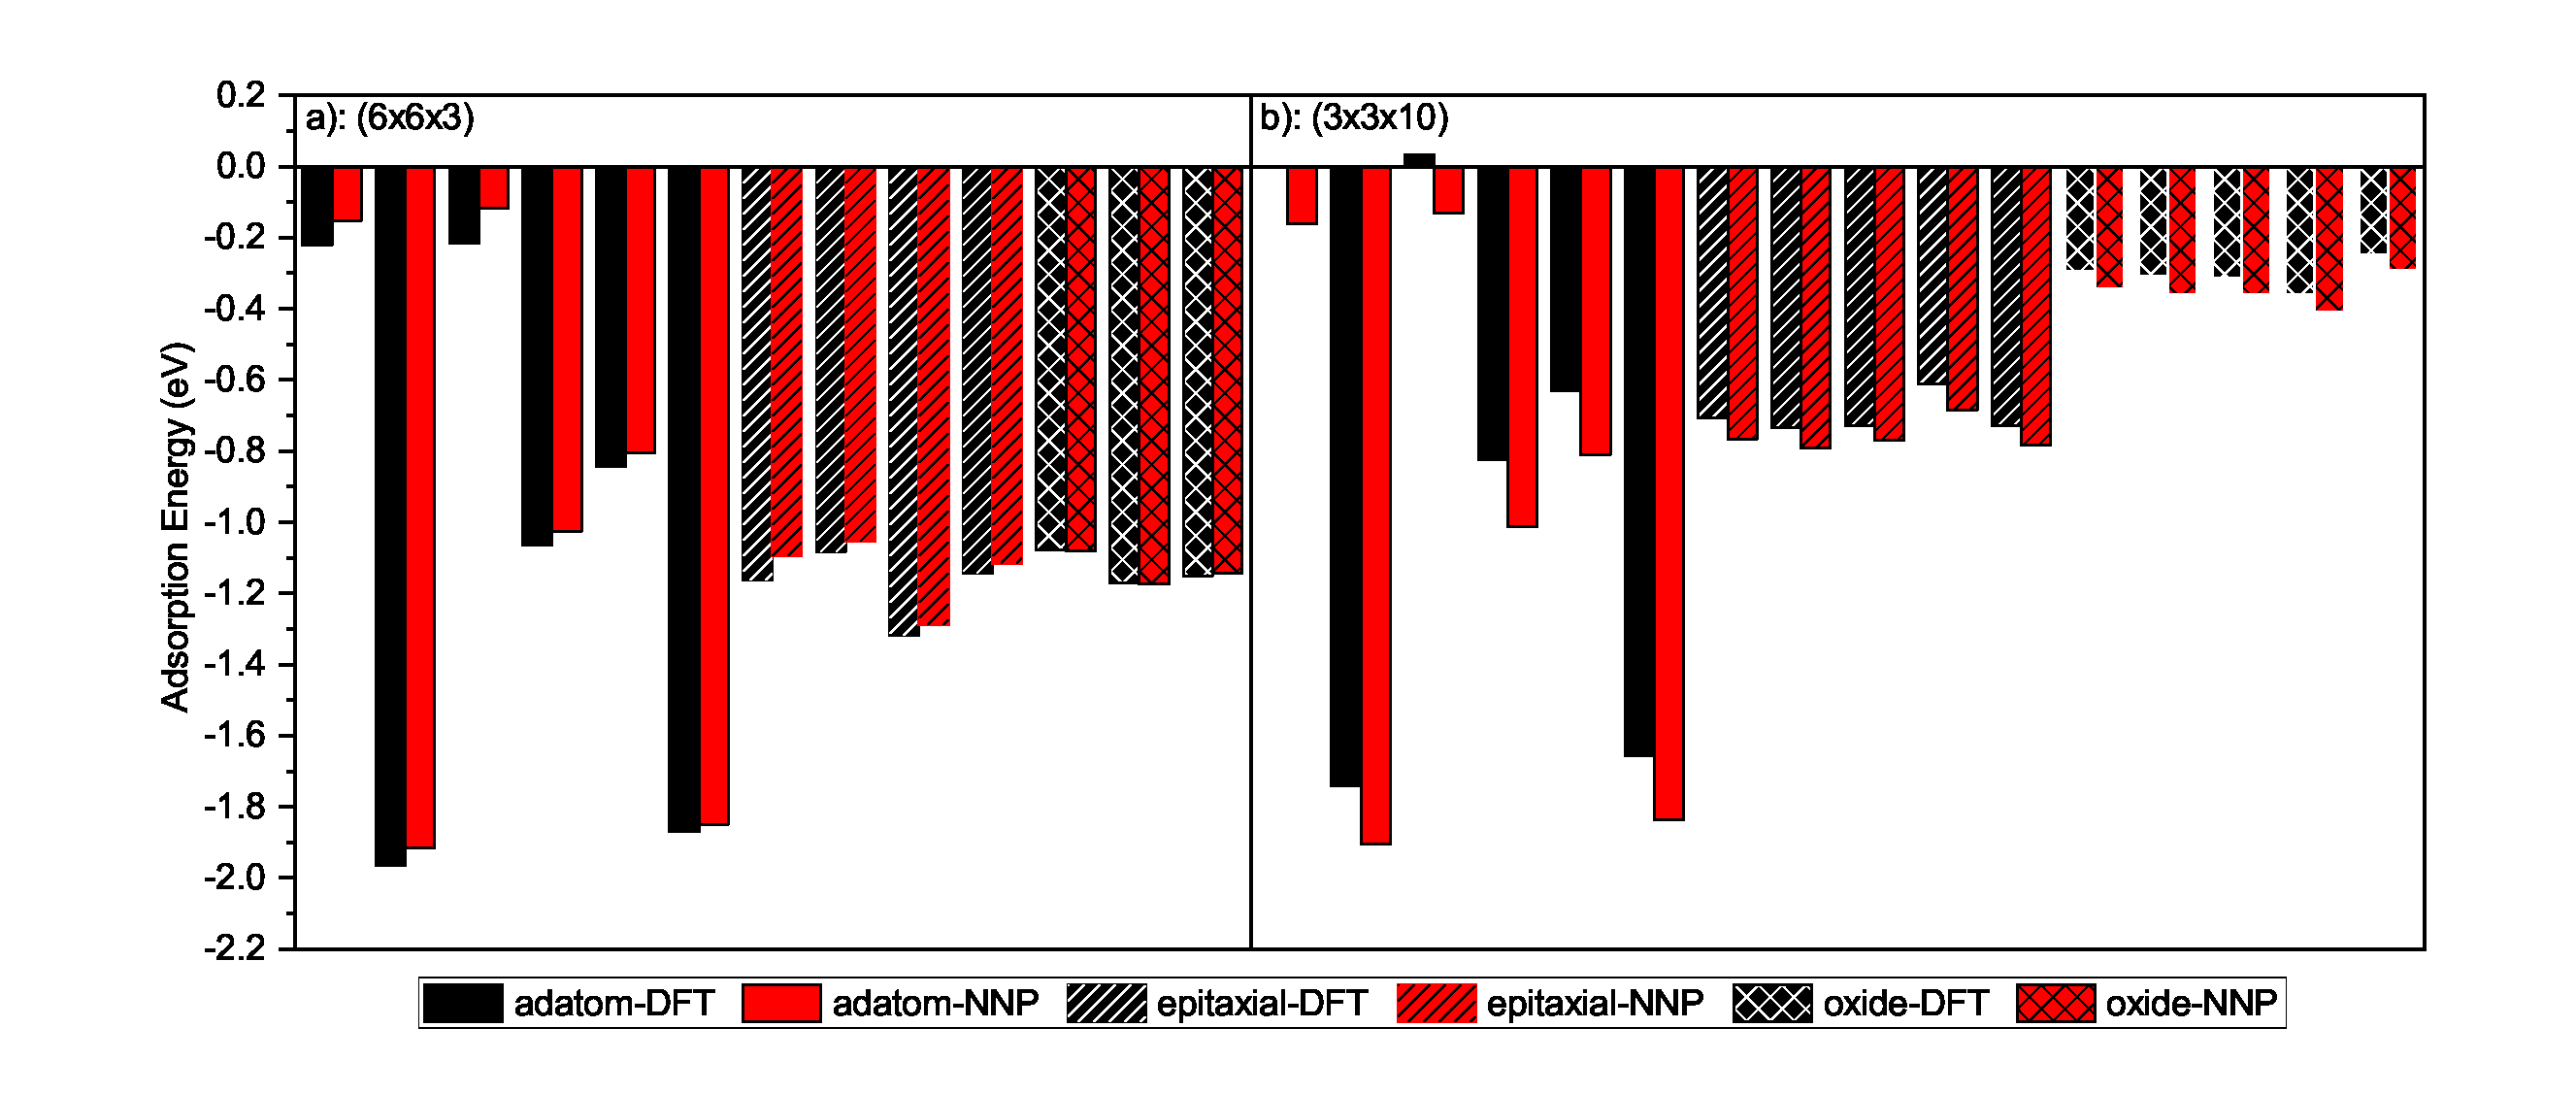
\includegraphics[width=\textwidth]{val_ads}
  \caption[Comparison of adsorption energies calculated using DFT and NNP]{Comparison of average adsorption energies on realistic test cases including single adatom adsorption, epitaxial oxide on metal, and fully oxidized slabs. \textbf{(a)}: result on a large ($(6\times6)$), thin (3 layer) \ch{Cu}(100) slab. \textbf{(b)}: result on a small($(3\times3)$), thick (10 layer) \ch{Cu}(100) slab.} 
  \label{fig:val_ads}
\end{figure}

The resulting network's performance on each sub-dataset is shown in Figure \ref{fig:subset}. It can be seen that all of the datasets have similarly low energy errors. The average adsorption energies on representative configurations from 3 different phases of oxidation are shown in Figure \ref{fig:val_ads}. Two types of slab structures are used: the $(6\times6\times3)$ slab and the $(3\times3\times10)$ slab. These structures are chosen as surrogates for the $(20\times20)$ production size slabs, since the latter is prohibitively expensive to calculate directly. Despite the adsorption being a stricter test than the error per atom, the final neural network performed remarkably well to give adsorption energies within \SI{0.1}{eV} for most of the configurations. In the worst case, the adsorption energy is within \SI{0.2}{eV} of the DFT value. We note that this accuracy is close to the inherent error in DFT itself.

As validation specific to our target plasma oxidation process, the potential energy surfaces that would be explored during the oxygen impact on the metal surface are probed by manually placing adsorbates at short distances above the pristine \ch{Cu} surface. Three surface sites (top, bridge, and hollow) are probed with atomic oxygen(\ref{fig:val_close}a), vertical (\ref{fig:val_close}b) and flat (\ref{fig:val_close}c) \ch{O2} molecules. The structures are illustrated in \textbf{SI}. Very good agreement between the DFT ground truth and the NNP prediction is found up to \SI{20}{eV} above the minimum energy adsorption height. These observations allow us to conclude that the neural network potential can reproduce \ch{Cu}-\ch{O} interaction for our purpose.

\begin{figure}[h]
  \centering
  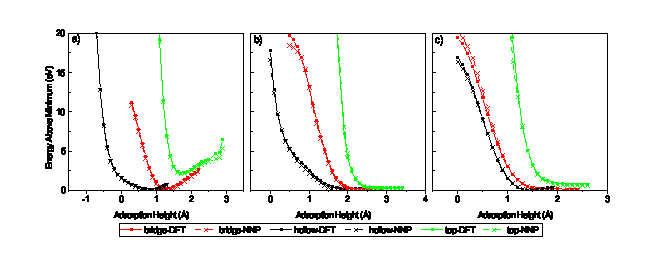
\includegraphics[width=\textwidth]{originprojects/closefig}
  \caption[Comparison of the PES calculated using DFT and NNP on simulated impact event]{Comparison of potential energy surfaces on short-distance, high-energy structures likely present in impact events. \textbf{(a), (b), (c)} are respectively for a single \ch{O} atom, a vertical \ch{O2} molecule, and a horizontal \ch{O2} molecule. The energies are plotted against the distance above the adsorption sites on a \ch{Cu} (100) surface.}
  \label{fig:val_close}
\end{figure}

\section{Results and Discussion}
With the trained and validated potential, large scale molecular dynamics simulations is performed. Figure \ref{fig:md_setup} shows the setup used to perform all the simulations presented in this section. Large slab structures of \ch{Cu}(100) are constructed from their DFT optimized bulk unit cell. These slabs have either square or nearly square unit cells with around \SI{3}{nm} length in each direction, and thick enough to ensure that the oxidation never reaches the bottom layers. To preserve the thermal spikes created by the plasma impact, only the regions near the edges are thermostated, as shown in Figure \ref{fig:md_setup} a). Hence, the atoms under the impact approximate the microcanonical ensemble, while the system as a whole approximate the canonical ensemble. The division of the vertical direction is shown in Figure \ref{fig:md_setup}b). During the simulation, the oxygen ions are added to the cell every \textbf{10000} steps, which roughly corresponds to \SI{5}{ps}, with a uniform $z$-velocity calculated from its specified kinetic energy, and the $x,y$-velocities calculated from the root mean square speed ($v_{rms}$) at the specified temperature. The neutrals addition frequency is set according to specification relative to the ion addition frequency, and all 3 velocity components are set to $v_{rms}$. Frequently, oxygen atoms recombine on the surface, and desorb as \ch{O2} molecules. These molecules are removed as soon as they reach the desorption region. No copper atoms are sputtered away from the substrate. 

\begin{figure}[h]
  \centering
  \includegraphics[width=0.7\textwidth]{mdsetup}
  \caption[Overall setup of MD simulations]{Overall setup of MD simulations. a) only the regions near the edge of the simulation box are thermostated. b) the vertical direction is divided into the desorption removal, new atoms addition, buffer, and the substrate regions}
  \label{fig:md_setup}
\end{figure}
% explain the 3 parameters
There are three variable parameters in the simulation with direct experimental significance: substrate thermostat temperature ($T_s$), ion kinetic energy ($E_k$), and the ratio of neutral to ions ($\gamma_{ni}$). The temperature corresponds well to the temperature of the wafer. The ion kinetic energy is affected simultaneously by the plasma power and the applied bias potential. The ratio of neutral atoms to ions is affected by the chamber pressure and the plasma power. While the quantitative relations between simulation parameters and experimental parameters are not known, the trend is clear: higher plasma power and higher pressure correspond to more, higher energy ions. 

In Figure \ref{fig:traj}, the evolution of the Cu(100) slab structures under $T_s=\SI{293}{K}$, $E_k=\SI{10}{eV}$, $\gamma_{ni}=10$ are shown. Changing these parameters does not affect the general stages of oxide growth which is discussed here. Starting with a pristine surface with a $20\times20$ surface supercell, both the ions and neutrals adsorb to form an overlayer of oxygen atoms. At this stage, the sticking coefficient $S$ is very high, and almost all the atoms added adsorb to the surface. As shown, the adsorption is not uniform on surface. The adsorbate ions tend to migrate between different sites initially, during which they impinge upon the copper atoms on the top layer and transfer the kinetic energy to the surface. Once their kinetic energies falls below the diffusion barrier on (100) surface, they settle down at a four-fold hollow site. The lateral interaction among the adsorbates are generally repulsive, leading to regions with c$(2\times2)$, p$(2\times2)$, and $(1\times1)$ configurations (Figure \ref{fig:traj}, $t=\SI{24}{ps}$). As the coverage is increased, the binding between the first layer of copper atoms to the layers underneath is weakened. Thus, copper atoms are lifted off the surface by thermal fluctuations, allowing oxygen atoms to migrate into the second layer. This process creates a corrugated surface, with islands of oxides and basins of pure copper (Figure \ref{fig:traj}, $t=\SI{56}{ps}$). The corrugation is significant in the growth of the oxide for two reasons. First, it allows the oxygen to migrate into the copper lattice before the active sites of adsorption is completely consumed. In Figure \ref{fig:traj}, $t=\SI{156}{ps}$, when the oxide is around 3 atomic layers thick there remains region on the surface not completely covered by oxygen. Second, the same process is be repeated at the interface between the oxide and the copper underneath: \ch{Cu}-\ch{O} binding weakens the binding of \ch{Cu} atoms to the copper lattice, lifts the \ch{Cu} atoms out , allowing oxygen atoms to diffuse through to the vacancy created.

% explain somewhere that the ion charges are not modelled explicitly. 
% show evolution of 1 100 slab
\begin{figure}[h]
  \centering
  \includegraphics[width=0.7\textwidth]{traj100}
  \caption[Snapshots along the oxidation trajectory of Cu(100) slab]{Snapshots along the oxidation trajectory of Cu(100) slab}
  \label{fig:traj}
\end{figure}
Beyond a few atomic layers, the growth of oxide slows down rapidly and transitions to a diffusion and/or interface reaction limited process, characterized by an amorphous copper oxide layer inert to further oxygen adsorption. The rate of oxygen incorporation decreases, and the rate of oxygen recombination and molecular desorption increases. Figure \ref{fig:thickness}a) shows the growth of oxide thickness with time, and Figure \ref{fig:thickness}b) shows the amount of oxygen incorporated into the slab. The details of characterizing this thickness from the MD trajectory is given in \textbf{SI}.

Comparing the results from the same temperature, there are clearly 2 regimes of growth: the fast regime at first, and the slow regime later. Two strands can be separated from the fast regime, each corresponding to different neutral-to-ion ratios, and independent of the kinetic energy of the ions. As the exposed adsorption sites becomes occupied, the growth slows down significantly. No limiting thickness is observed. Instead, the oxides continue to grow at a slow rate of around \SI{0.15}{nm/fs}. The growth rate in this regime seem to be determined by $E_k$, where the thickness profiles gradually separate into two strands dintinguished by a faster growth at the larger $E_k$ of \SI{20}{eV} against the slower growth at \SI{10}{eV}.

The effect of substrate thermostat temperature $T_s$ can also be seen by comparing curves with same line color and symbol, but with different symbol colors. Higher substrate temperature is seen to promote oxide growth by postponing the transition to the slower regime. Its effect is similar to but less pronounced than that of the ion kinetic energy. 

\begin{figure}[h]
  \centering
  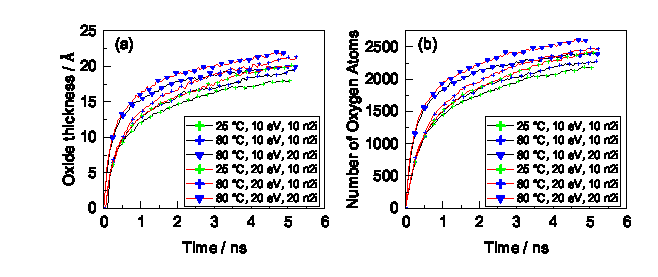
\includegraphics[width=\textwidth]{fig_thicknumo_100}
  \caption[Evolution of oxide thickness]{Evolution of oxide thickness}
  \label{fig:thickness}
\end{figure}

The two regimes can be rationalized by considering the physical processes at work. Initially, when the pristine surface is exposed to oxygen plasma, the high-energy ions have a large free energy driving force to adsorb. Hence, we expect all the impinging ions to adsorb. Moreover, the ions do not have enough kinetic energy to penetrate even the first layer. In Figure \ref{fig:traj}, from the first snapshot, it can be observed that all of the oxygen atoms are stopped at the top layer. Therefore, the kinetic energy of the ions are transferred to the \ch{Cu} lattice and dissipated via lattice vibrations into the bulk copper. In the simulation, they dissipiate to the thermostated regions, without creating lattice or surface defects in the process. 

As the oxide grows, less and less low-coordinated surface \ch{Cu} atoms are exposed, driving down the sticking coefficient. The oxide growth becomes more and more limited by the migration of \ch{O} atoms into the \ch{Cu} lattice, and the oxidation reaction at the oxide-metal interface. Both reactions are limited by the energy available to the oxygen atoms at the interface to overcome the energy barrier. In the thermal oxidation process, the only source of energy would be the random thermal fluctuations. Hence, we would expect the growth rate to depend mainly on the substrate (thermostat) temperature. In a plamsa-enhanced process, the impinging ions act as additional source of thermal energy. The thermal spikes created by the ions propagate through the oxide layer and the \ch{Cu} lattice, elevating the kinetic energies of atoms in its path. Each step along the collision cascade, only a fraction of the energy is transferred to the next atom in the layer underneath. The thermal spike heats up the atoms along the path of its cascade to kinetic energies of several orders of magnitudes higher than the Maxwell-Boltzmann distributed thermal fluctuations would allow. Such high energies would overcome reaction barriers easily. However, as we demonstrate below, such highly concentrated energy is only available to atoms within a few layers of the impact event, due to the fast dissipation. This is especially the case of the amorphous copper oxide layers, where non-symmetric environment means that neighboring atoms do not always exist in the direction of propagation, hence the energy is more likely to dissipate.

To explore this point further, individual impact simulations on pristine \ch{Cu} surfaces and a oxide surface are performed with fast ions only (no slow neutrals), and the maximum of the depths of atoms agitated by the heat spikes are calculated and gathered in Figure \ref{fig:spikes}. The penetration depth is defined as the depth of the deepest atom that has a kinetic energy with probablities less than $f_{cut}=1\times10^{-5}$ in the Maxwell-Boltzmann distribution, and connected via a series of collision events to the impact site. At \SI{10}{eV}, the heat spike never exceeds \SI{12}{\AA}, corresponding to 5 layers in the copper slab. Increasing the kinetic energy to \SI{20}{eV} nearly doubles the penetration depth. On the \ch{Cu} copper surface, the distribution shows discreteness due to the well-defined layers in crystalline structure. On the amorphous oxide layer, the increase in penetration depth is less pronounced as discussed above, but increasing kinetic energy gives a larger spread in depth profile. Note that the numeric value of the spike depth does not have significance as it relies sensitively on the choice of $f_{cut}$, and the implemented collision event tracking method (see \textbf{SI}). Nevertheless, the qualitative trend is clear: as the kinetic energy is increased, the thermal spikes are able to excite more atoms, and reach deeper down the surface. This observation is reminiscent of the ion implantation technique, where both the projected range and the straggle increase as kinetic energy is increased. Thus, the ions serve as a transient, anisotropic, high intensity energy source to help thermally activate the oxidation reaction. This in contrast to the thermal energy which is persistent, isotropic, and low intensity. 

\begin{figure}[h]
  \centering
  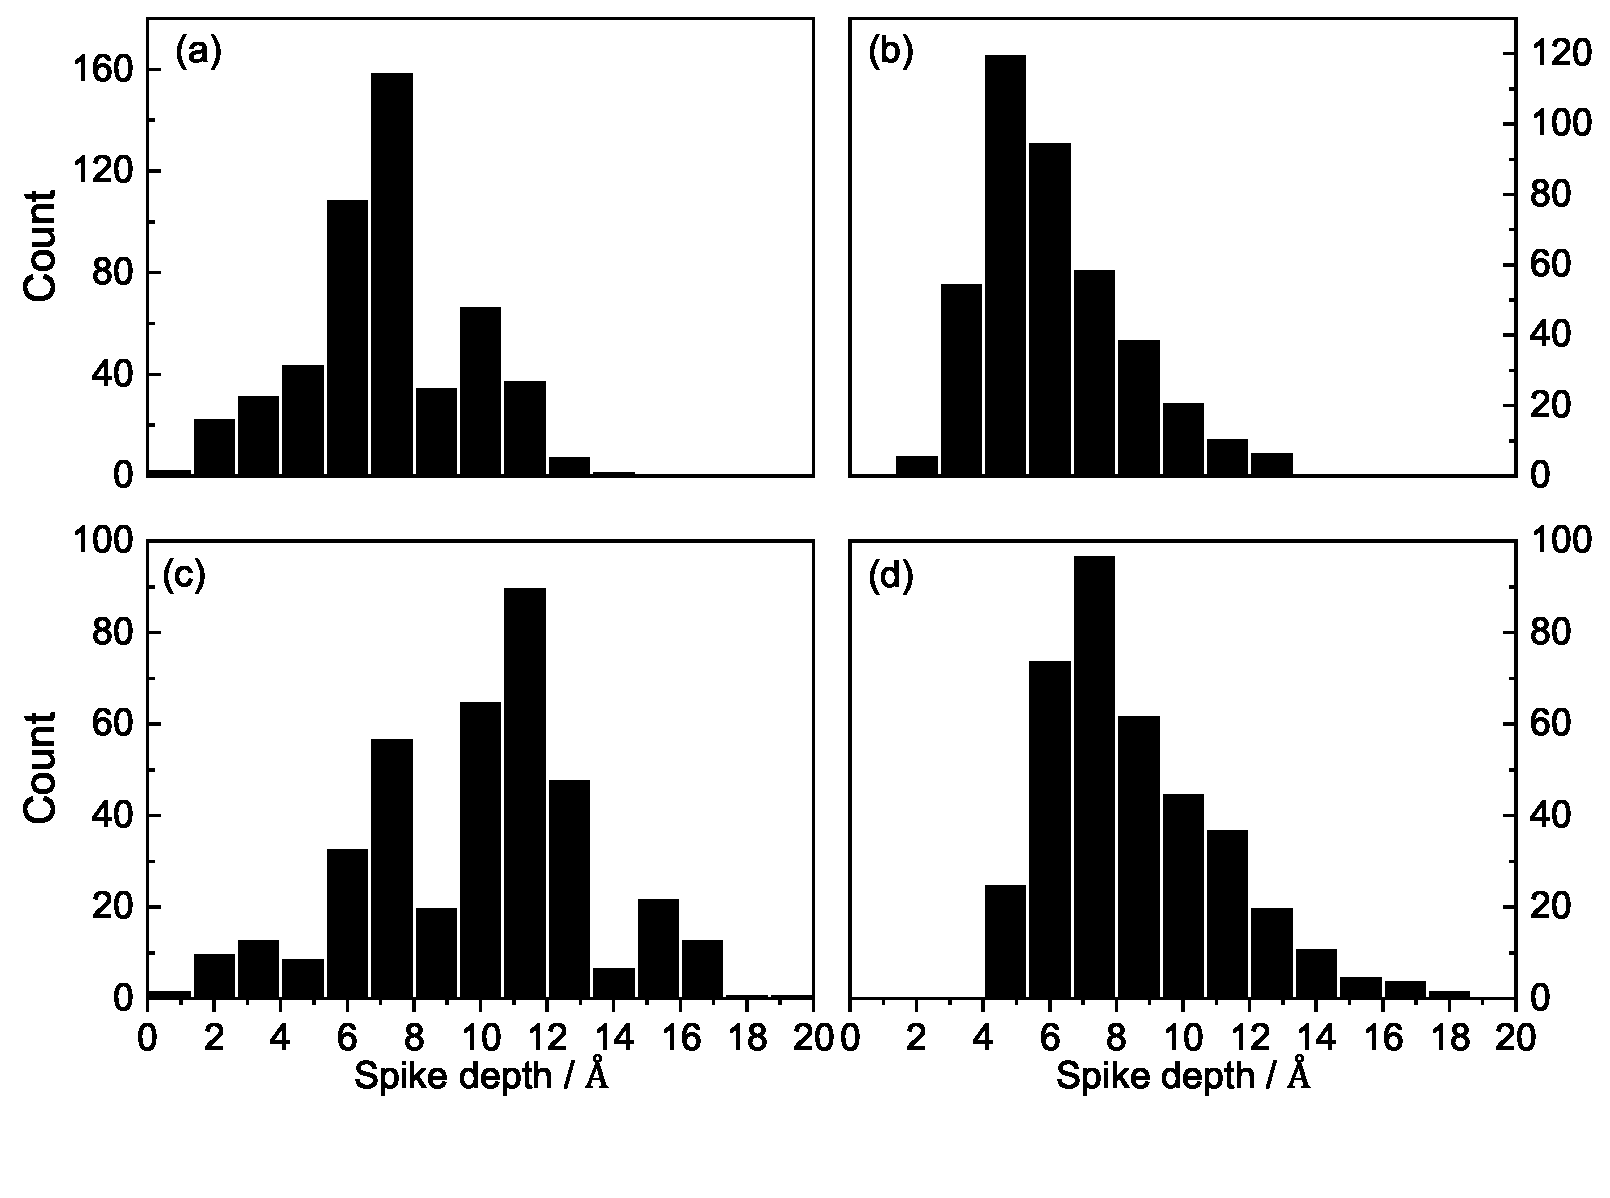
\includegraphics[width=\textwidth]{spikes}
  \caption[Distribution of penetration depths on Cu]{Distribution of penetration depths on Cu (100), and \ch{CuO} slabs.}
  \label{fig:spikes}
\end{figure}

Based the distinct nature of heat sources, a third regime is likely to be present where the growth rate is determined by the substrate temperature. However, our simulation cannot be extended long enough to discern this regime clearly. If our rationale holds, this temperature-limited regime will be present when the oxide grows beyond the thickness affected by the thermal spikes. As a word of caution, note that the \SI{6}{ns} of simulation time covered has no correspondence to experimental time, since the deposition rate is much higher than what is likely under the experimental pressures (see comparison in \textbf{SI}).

%%% We do not have saturation thickness: %%%
% Also note that the saturation thickness does not necessarily correspond to the experimental oxide thickness, since the much slow diffusion process cannot be properly accounted for at this time scale.

%%% the structure of the results section: %%%
% 1. an overview of oxidation, the large scale simulation with atomic resolution
% 2. the trends of thickness and oxygen incorporation
% 3. on average, the phase of the oxide formed
% 4. more detailed atomistic information on the oxide (conc. grad. and the crystalline regions)
% 5. observed temperature gradient
% 6. fitting of this temperature gradient to growth rate, and the prediction thereof
% 7. relative magnitude of diffusion activation energy and the apparent activation energy
% 8. feature-scale simulations (COMSOL)

%%% To add: %%%
% 1. the temperature gradient stuff
% 2. the concentration gradient
% 3. the brute-force fitting
% 4. the diffusion stuff

\begin{figure}[h]
  \centering
  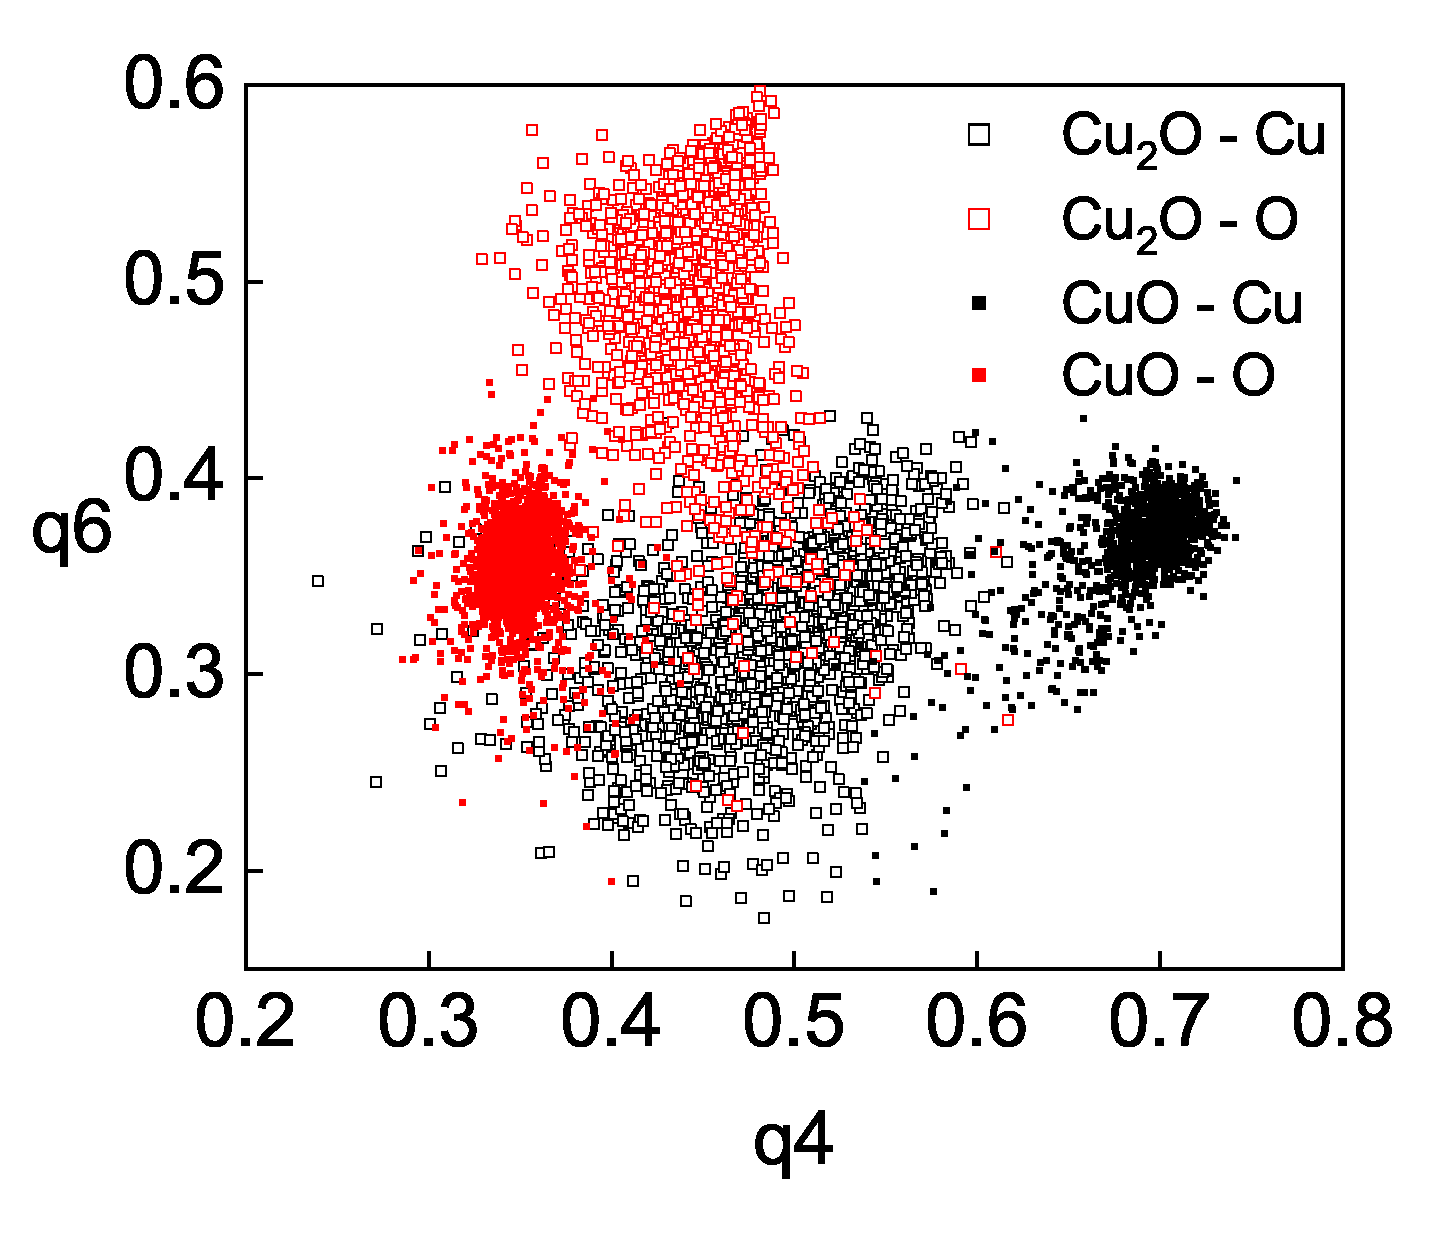
\includegraphics[width=0.5\textwidth]{cuo_id.eps}
  \caption[Bond orientational order parameter for bulk]{Bond orientational parameters for bulk \ch{CuO} and \ch{Cu2O}}
  \label{fig:cuo_id}
\end{figure}

Next, we applied the Voronoi tessellation averaged bond orientational order (BOO) parameters to study the crystal structure of the seemingly amorphous copper oxide layers. Shown in Figure \ref{fig:cuo_id}a) is the resulting $\bar{q}_4$ and $\bar{q}_6$ parameters for high-temperature MD of supercells of the two copper oxide crystals \ch{Cu2O} and \ch{CuO}. The two structures are clearly distinguishable on this figure. \ch{CuO} has two clusteres with similar $\bar{q}_6$ parameter values around $\sim$ 0.40, but different $\bar{q}_4$ values at $\sim$ 0.35 and $\sim$ 0.70, corresponding to \ch{O} and \ch{Cu} atoms, respectively. On the other hand, \ch{Cu2O} have two clusters with similar $\bar{q}_4$ values at $\sim$ 0.50, but different $\bar{q}_6$ values centered at $\sim$ 0.5 and $\sim$ 0.3, respectively for \ch{O} and \ch{Cu}. 
\begin{figure}[h]
  \centering
  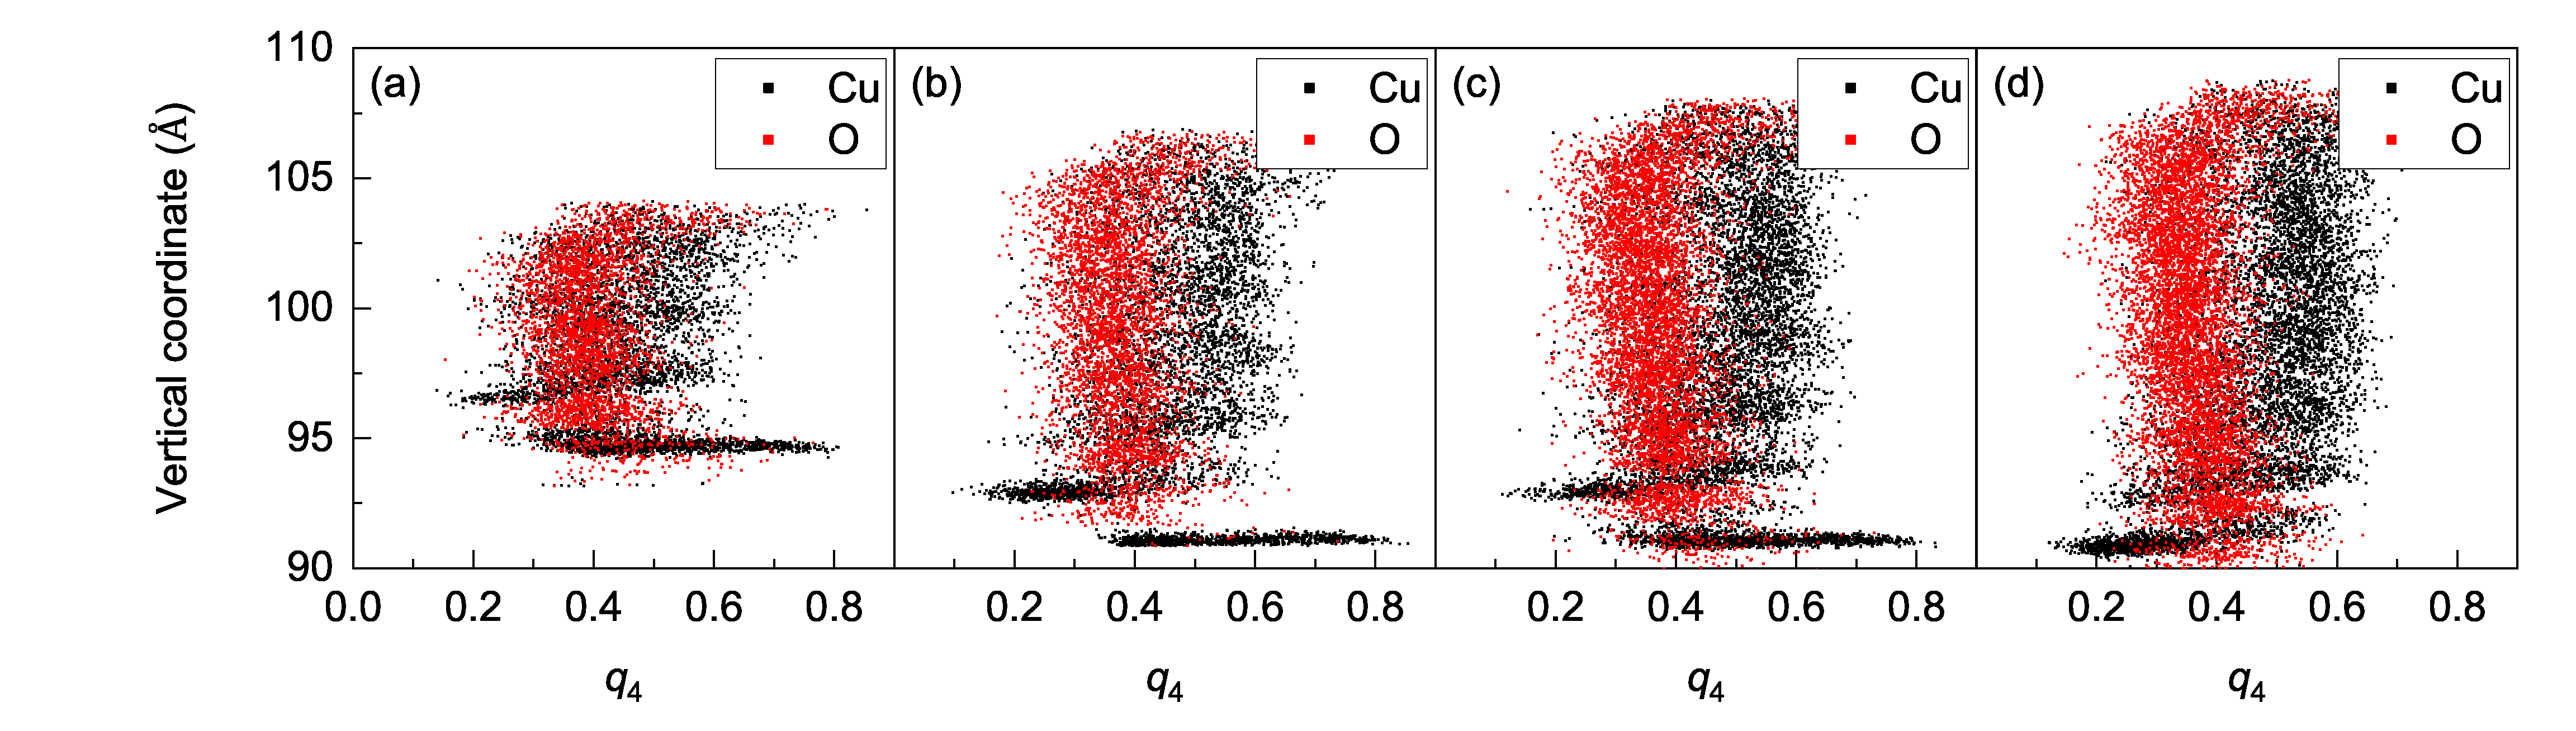
\includegraphics[width=\textwidth]{boo_1234.eps}
  \caption[Steinhardt's order parameter for slab]{Bond orientational order parameter $\bar{q}_4$ (Voronoipp tessellation averaged) for range of oxide thicknesses. }
  \label{fig:boo_slab}
\end{figure}

In Figure \ref{fig:boo_slab}, the calculated BOO parameter are plotted against their vertical coordinate ($z$-coordinate). For clarity, only $\bar{q}_4$ is shown. The $q_6$ parameters of \ch{Cu} and \ch{O} overlap each other and can be found in the \textbf{SI}. The structures used in Figure \ref{fig:boo_slab} are extracted from $T_s=\SI{353}{K}, E_k=\SI{10}{eV}, n/i = 10$ simulations and re-equilibrated at $\SI{353}{K}$ to remove thermal spikes that may have resulted from recent impact events. The structures clearly illustrate the growth of an oxide-like local environment, distinct from the layered pristine copper atoms towards the bottom of each panel. Furthermore, the parameters indicate the dominance of local \ch{CuO}-like environment, as indicated by the segregation of $\bar{q}_4$ parameters derived from \ch{Cu} and \ch{O} into respectively clusters at values of 0.3 and 0.6, respectively. Such segregation is not observed in the very thin oxide of Figure \ref{fig:boo_slab} (a), but only becomes pronounced as the thickness increased. The position of the clusters stabilize beyond thicknesses of \SI{2}{nm}. Comparison with the Figure \ref{fig:cuo_id} suggests the resulting oxide after long exposure to oxygen plasma will have the structure and composition of \ch{CuO}. This result is consistent with experimental X-ray photoelectron spectroscopy study, although in that case the \ch{Cu2O} polymorph is not ruled out. The overall stoichiometry of the oxide film is very close to 1, agreeing with the local environment analysis. 

In Figure \ref{fig:boo_slab}, the point clouds of \ch{Cu} and \ch{O} atoms clearly cluster in the $(\bar{q}_4-\bar{q}_6$ plane. Additionally, there is hints of clustering in the $z$-coordinate as well. Unable to carry out the simulation to very long time scales due to size of the structures involved ($\sim$ 20000 atoms), similar MD simulations were performed on the smaller $(10\times10)$ \ch{Cu} (100) slab ($\sim$ 5000 atoms) to exploit the higher effective ion flux and lower computational cost per step. When the neutrals are turned off, and all oxygen deposits are the fast ions, the resulting BOO parameters are in Figure \ref{fig:10x353K10n2i_comp}b show clustering in the z coordinate. The structure itself shows almost crystalline \ch{CuO} motifs within $\sim$ 5 layers above the oxide-metal interface, as also captured by the BOO parameter. Above the crystalline region, the film is amorphous and porous, due to repeated high-energy influx from oxygen impacts. The segregation in $z$ allows DBSCAN clustering to be performed on the clusters, and the centers of mass of the resulting clusters are given in Table \ref{tab:cluster_com}. From the clustering analysis, we confirm that at least the local environment closely resembles \ch{CuO}. Note that the BOO parameters from atoms at the surface is unreliable, due to the tendency of the Voronoi tessellation definition of neighbors to overestimate the number of neighbors. This causes the large spread near the top of the oxide slab seen in Figures \ref{fig:boo_slab,fig:10x353K10n2i_comp}. 

% evolution of these clusters in time
\begin{figure}[h]
  \centering
  \includegraphics[width=\textwidth]{10x353K10n2i_comp}
p  \caption[Steinhardt's order parameter for slab]{BOO parameter on $(10\times 10)$ \ch{CuO} (100) slabs and the corresponding structure.}
  \label{fig:10x353K10n2i_comp}
\end{figure}
\begin{table}[h]
  \centering
  \caption[test]{Centers of clusters in Figure \ref{fig:10x353K10n2i_comp}}
  \begin{tabular}[c]{cccc}
    \thead{$q_4$} & \thead{$q_6$} & \thead{z-coordinate / \AA} & \thead{Element} \\ \hline
    0.56 & 0.35 &  94.12 & Cu\\
    0.61 & 0.37 &  96.70 & Cu\\
    0.61 & 0.37 &  99.29 & Cu\\
    0.60 & 0.38 & 101.80 & Cu\\
    0.59 & 0.38 & 104.34 & Cu\\
    0.36 & 0.37 &  95.41 & O \\
    0.34 & 0.35 &  98.00 & O \\
    0.33 & 0.34 & 100.50 & O \\
    0.33 & 0.34 & 103.06 & O \\
    0.34 & 0.33 & 105.61 & O \\
  \end{tabular}
  \label{tab:cluster_com}
\end{table}

Next, we investigated the internal structure of the oxide film formed. Shown in Figure \ref{fig:conc_grad} is the atomic concentrations of \ch{O} and \ch{Cu} atoms as a function of thickness. These profiles, while noisy, shows two characteristics: the oxide film can be considered to have 2 parts: a porous region within $\sim \SI{1}{nm}$, indicated by the lower overall density, and a dense region beyond this thickness. In the dense region, a clear gradient of oxygen and copper concentration can be seen. It is emphasized that the observed gradient is not a result of uneven oxidation front: the onset of the gradient, at $\sim\SI{8}{\AA}$ above the oxidation front (as defined in \textbf{SI}), is completely within the oxide. The existence of such gradients indicate that diffusion is a possible activated process, in addition to the oxide/metal interface reaction.

To study the thermal activation of diffusion inside the oxide, the diffusivities at temperatures \SIrange{200}{1000}{K} are calculated (see details in \textbf{SI}), and fitted to an Arrhenius type relation. As shown in Figure \ref{fig:DvT}, the diffusivities follow the Arrhenius relation well, indicating an activation energy of \SI{0.00}{eV}. 

To ensure our results is not particular to the \ch{Cu} (100) slab, we have performed similar simulations on the \ch{Cu} (111) surface. Figure \ref{fig:traj111} shows the evolution of the (111) surface, and Figure \ref{fig:thicknumo_111} shows the thickness and oxygen content as functions of simulation time. Note that the surface cell is orthogonalized to make LAMMPS setup easier, and the noise is considerably higher due to the smaller number of atoms used. The surface undergoes similar stages of oxidation. The thickness of the oxide is similar to that on (100) under similar operation conditions. The clusters of Steinhardt's parameters are also similar to those found on (100) surfaces (see Figure \textbf{S}). Since (111) and (100) are the low-energy surfaces exposed in equilibrium conditions, we expect our result to be generally valid. This is also reasonable from our plasma oxidation theory: if the oxide thickness is essentially limited by the penetration depth of the thermal spike in the oxide layer, and the oxide layer is for the most part amorphous, then the substrate orientation should not have significant effect on the simulated oxide thickness. In reality, the crystal orientation will likely affect the slower diffusion process. However, as indicated earlier, our model does not treat the thermal diffusions explicitly. 
% 111 and copper oxide transformation, do not have it yet. 

\begin{figure}[h]
  \centering
  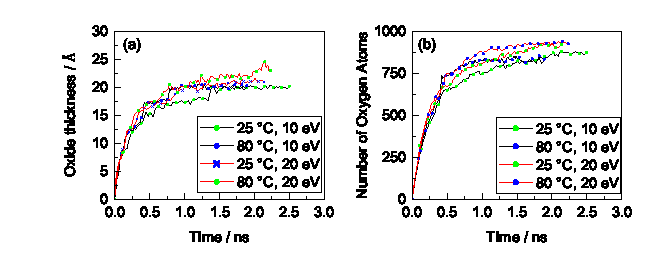
\includegraphics[width=\textwidth]{thicknumo_111.eps}
  \caption[Steinhardt's order parameter for slab]{Thickness and number of oxygen in the growing oxide on \ch{Cu} (111) surface. }
  \label{fig:thicknumo_111}
\end{figure}

\begin{figure}[h]
  \centering
  \includegraphics[width=\textwidth]{traj111}
  \caption[Oxidation trajectory on the Cu (111) surface]{Oxidation trajectory on the Cu (111) surface}
  \label{fig:traj111}
\end{figure}

Lastly, we propose the following strategy to achieve self-limited oxidation layer in plasma processing. Because oxidation, as we have demonstrated, is mostly a diffusion limited process. To contain a diffusion process to the surface, the substrate temperature itself should be lowered to where diffusion practically stops during the processing time window. Then, the thickness is tuned by varying the plasma power, which affects the kinetic energy of the ions, and in turn the penetration thickness of the thermal spike. The thickness of the oxide created, will be self-limiting in the sense that it only depends on the kinetic energy, but not on the exposure time. Depending on application, this may or may not be feasible in an ALE process, since the subsequent removal step requires in general higher temperatures to facilitate etching product desorption. Nonetheless, using lower oxidation temperature during oxidation will likely improve the precision of patterns, at the potential expense of throughput. 

\section{Conclusions}
A novel machine learning potential is developed for the \ch{Cu}/\ch{O} system that covers atomic and molecular adsorption with initial kinetic energies upto \SI{20}{eV}. The potential is applied to study the plasma oxidation of copper, and the results demonstrate that the oxidation is a diffusion-limited process that produces \ch{CuO}. The observed oxidation trajectories are explained in terms of the avaiable energies to overcome diffusion barriers. The sources of such energy are identified. The immediate consequences for creating a self-limited oxidation process is that low-temperature substrate should be used whenever possible. The thickness can then be controlled via plasma power. 
\bibliography{ref}    % bibliography references
\end{document}

%%% Local Variables:
%%% mode: latex
%%% Tex-engine: xetex
%%% TeX-master: t
%%% End:
